% % % % % % % If you have a single appendix, you should be using appendix1.tex
% % % % % % % NOT this file

\chapter{Orthonormal Basis Functions and Mercer's Theorem}
\label{a:mercers_theorem}

Given an RKHS $\clH$, it is useful to understand the set of functions that belong to the Hilbert space. This can be studied using Mercer's theorem \cite{merrus09}. Mercer's theorem forms the connection between the theory of reproducing kernels and integral operators. 
Consider the integral operator (Hilbert-Schmidt operator) $L_K:L^2_\measure(x) \to L^2_\measure(x)$ defined by,
\begin{equation}
(L_K f)(x) = \int_\state \Kern(x,t) f(t) d\measure(t)
\end{equation}
where $\measure$ is a finite Borel measure and $\state$ is a compact set.
The linear map $L_K^{1/2}$, which denotes the square root of $L_K$ is a Hilbert isomorphism between $L^2_{\measure}(\state)$ and $\clH$ as illustrated in \Fig{fig:rkhs_isomorphism}. 

\begin{figure}[htbp]
	\centering
	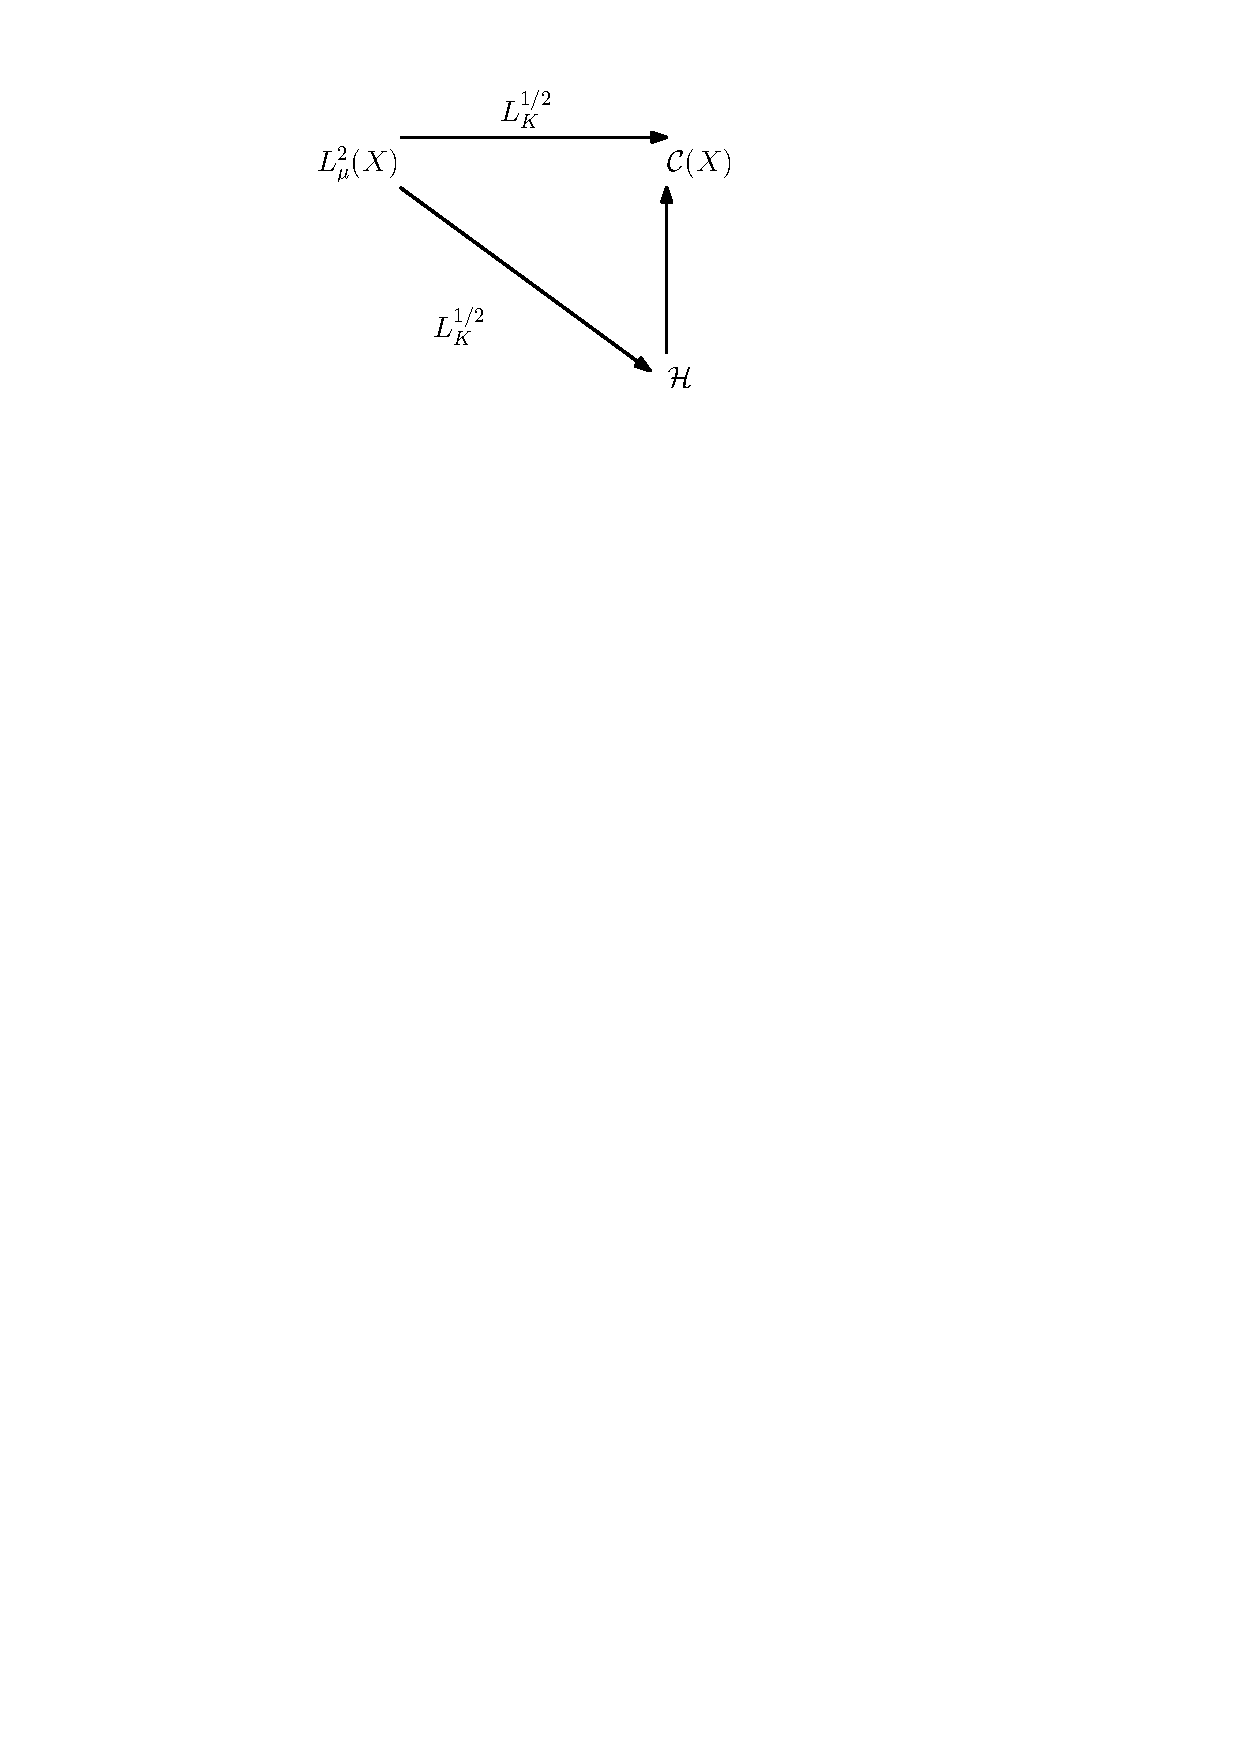
\includegraphics[width=3in]{images/Chap3_RKHS_isomorphism}
	\caption{Diagram illustrating the isomorphic transformations between $\clH$ and $L^2_\measure$.}
	\label{fig:rkhs_isomorphism}
\end{figure}

% $L_{K,C}$ emphasizes that the target is $\mathcal{C}(\state)$ and $I_K$ denotes the inclusion. If $\Kern$ is $\mathcal{C}^\infty$, then $I_K$ is compact. \anand{Gaussian kernel is $\mathcal{C}^\infty$}
$L_K$ is a self-adjoint, compact operator with eigenvalues $\reg_1 \geq \reg_2 \geq \cdots \geq 0$, with the corresponding normalized eigenfunctions $\{\phi_n\}_{n=1}^\infty$ forming an orthonormal basis for $L^2_\measure(\state)$. Mercer's theorem states that 
\begin{equation}
\Kern(x,x') = \sum_{n=1}^\infty \reg_n \phi_n(x) \phi_n(x'),
\end{equation}
where the series converges absolutely for each $x,x' \in \state$. The set $\{\sqrt{\reg_n}\phi_n\}_{n=1}^\infty$ forms an orthonormal basis for $\clH$. However, finding an eigenfunction feature representation for a kernel is challenging, except in special cases. 
